\section{Materiales y métodos}

\subsection{Materiales}
Los genes relacionados con el fenotipo ``Maternal diabetes'' (HP:0009800) fueron extraídos de la base de datos Human Phenotype Ontology (HPO) en la web hpo.jax \cite{Kohler2017}. Específicamente, se trabajó con una lista de 43 genes asociados al fenotipo, la cual se encontraba en formato excel.

Se utilizaron las librerías de Python
%La API de StringDB \cite{Szklarczyk2015} como la herramienta principal.
openpyxl 3.1.2, Stringdb 0.1.5 \cite{Mering2005}, Pandas 2.1.2 \cite{McKinney2015}, iGraph 0.11.2 \cite{Csardi2006} y Cairocffi 1.6.1, para el procesamiento de datos y las representaciones.

%La configuración e instalación necesarias se llevaron a cabo mediante scripts en Bash \cite{Dong2023}.

Ejecutado en un MacBook Air 15 con Intel Core i5-5250U CPU 1.60GHz, 8 GB RAM y sistema operativo Ubuntu 22.04.3 LTS (Jammy Jellyfish).

\subsection{Metodología}

EL flujo de trabajo que se siguió puede observarse en la figura \ref{fig:workflow} y que se explicará en detalle a continuación.

\begin{figure}[h!]
	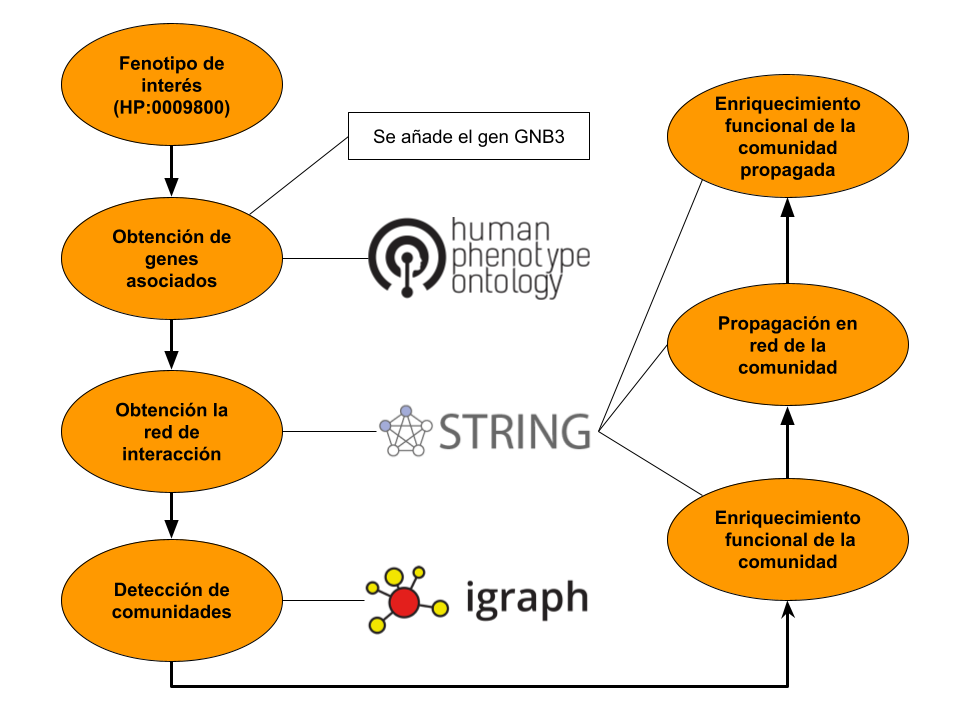
\includegraphics[width=0.9\textwidth]{figures/workflow.png}
	\caption{Flujo de trabajo: Se representa el flujo de trabajo seguido para la realización del proyecto. Empieza desde la obtención de los genes asociados al fenotipo de interés y la creación de la red de interacción hasta el análisis por enriquecimiento funcional.}
	\label{fig:workflow}
\end{figure}

Descargamos la lista de genes implicados al fenotipo HP:0009800 directamente desde HPO en formato xlsx e insertamos en la lista el gen GNB3 (id = 2784).

Utilizamos la librería stringdb de Python para obtener la red de interacción de los genes asociados al fenotipo.

Mediante la librería de igraph se construyó la red de interacción de genes y se realizó un algoritmo de detección de comunidades basado en ``edge betweenness'' \cite{Girvan2002}. Una vez realizada la detección, se seleccionó la comunidad donde estaba presente el gen GNB3.

Realizamos un enriquecimiento funcional de los genes que formaban parte de esa comunidad con la librería de stringdb y filtramos el resultado para quedarnos con las filas donde aparece GNB3. 

Se creó una nueva red mediante una propagación en red de los genes presentes en la comunidad de interés con el parámetro ``add\_nodes = 16''. A partir de esta red volvimos a realizar un enriquecimiento funcional.